\documentclass{article}
\usepackage[UTF8]{ctex}
\usepackage[tc]{titlepic}
\usepackage{titlesec}
\usepackage{cite}
\usepackage{fancyhdr}
\usepackage{booktabs}
\usepackage{graphicx}
\usepackage{geometry}
\usepackage[section]{placeins}

\usepackage{amsmath}
\usepackage{cases}
\usepackage{color}
\usepackage{hyperref}
\hypersetup{hypertex=true,
	colorlinks=true,
	linkcolor=blue,
	anchorcolor=blue,
	citecolor=blue}
\usepackage{listings,xcolor}
\usepackage{multirow}
\usepackage{tabularx}
\usepackage[utf8]{inputenc}

\usepackage{cleveref}
\crefname{section}{\S}{\SS}
\Crefname{section}{\S}{\SS}

\geometry{a4paper,scale=0.8}
\pagestyle{fancy}

\usepackage{dirtree}
\usepackage{caption}

\lhead{\today}
\chead{中国科学技术大学\\大数据系统及综合实验课程}

\rhead{{\CTEXoptions[today=old]\today}}
\newcommand{\upcite}[1]{\textsuperscript{\cite{#1}}}

\titleformat*{\section}{\bfseries\Large}
\titleformat*{\subsection}{\bfseries\large}
\titleformat{\section}[block]{\Large\bfseries}{\S \thesection}{0em}{}

\title{\bfseries 基于Hbase的USTC官方文件查询系统}
\author{殷腾 \quad PB20030785\\
	李新涛 \quad PB21151754}

\begin{document}
	\maketitle
	%\clearpage
	% \setcounter{secnumdepth}{1}
%	\setcounter{section}{-1}
%	\clearpage
	\begin{abstract}
		本项目基于Hbase数据库,实现了一个USTC官方文件查询系统。
		通过预先爬虫爬取USTC官方网站的文件,将文件存储在Hbase数据库中,并提供了一个简单的界面供用户查询。
		用户可以通过关键词检索文件,系统将返回相关文件的信息。
		系统支持对文件信息的排序,用户可以根据搜索词与文件关联性对文件进行排序。系统还支持对文件的下载,用户可以通过界面下载文件到本地进行查看。
		系统的实现主要分为数据库与界面等部分。系统的实现过程中,我们使用了Python语言,Hbase数据库,PyQt5等工具。
		最终系统的实现效果良好,用户可以通过界面方便地查询、下载USTC官方文件。
	\end{abstract}

	\tableofcontents
	\clearpage
	
	
	\section{项目简介}
	本项目基于Hbase数据库,实现了一个USTC官方文件查询系统。
	通过按照一定格式爬取文件后,系统会将其存储在Hbase数据库中。
	用户可以通过系统提供的图形化界面输入关键词,系统将返回相关文件的信息。
	用户可以通过界面查看文件的信息,并下载文件到本地进行查看,避免了用户在USTC官方网站上进行繁琐的查找。

	\section{项目框架}
	\subsection{界面}
	界面使用PyQt5实现,主要包括一个检索输入框和结果展示列表。当用户输入关键词后,系统会在Hbase数据库中检索相关文件,并将相关文件的各项信息结果展示在列表中。
	同时列表中的结果支持直接下载,用户可以通过点击列表中的文件名下载文件到本地进行查看。
	除此之外,若用户输入的关键词为空或者无相关文件,系统会给出提示信息。
	
	\subsection{检索}
	检索功能主要通过Hbase数据库实现,使用Python第三方库happybase连接Hbase数据库。
	系统会在Hbase数据库中检索相关文件,将检索到的文件信息返回给用户。
	检索功能支持对文件信息的排序,用户可以根据搜索词与文件关联性对文件进行排序。
	
	\section{细节实现}
	\subsection{爬虫}
	爬虫主要使用Python第三方库requests、BeautifulSoup实现,爬取USTC官方网站的文件。
	本次实验中主要选取了人工智能与数据科学学院、计算机科学与技术学院、数学科学学院、网络空间安全学院、
	信息科学技术学院、软件学院、财务处、出版社、学位与研究生教育、财务处这十个学院的官方文件进行爬取。
	\\
	\indent 由于一些网站本身的文件数量就很少,使用爬虫收益太低,所以我们选择手动下载这些学院的文件。此外,我们还尝试使用了IDM中的站点爬取功能,获取了未被列举在文档中心的doc、docx、xls、xlsx类型文件,总计894个文件。
\newpage
	\subsection{建表}
	考虑到在使用校内文件搜索时,不同学院的学生会有不同的需求,即对于某一项规定,不同学院学生可能会有不同的要求。因此,在建表时,除了必要的文件名、数据这两项属性外,还增加了来源机构这一属性。而考虑到不同学院可能会存在同名的文件,选择(文件名\_来源机构)作为row\_key。
	\begin{figure}[h]
		\centering
		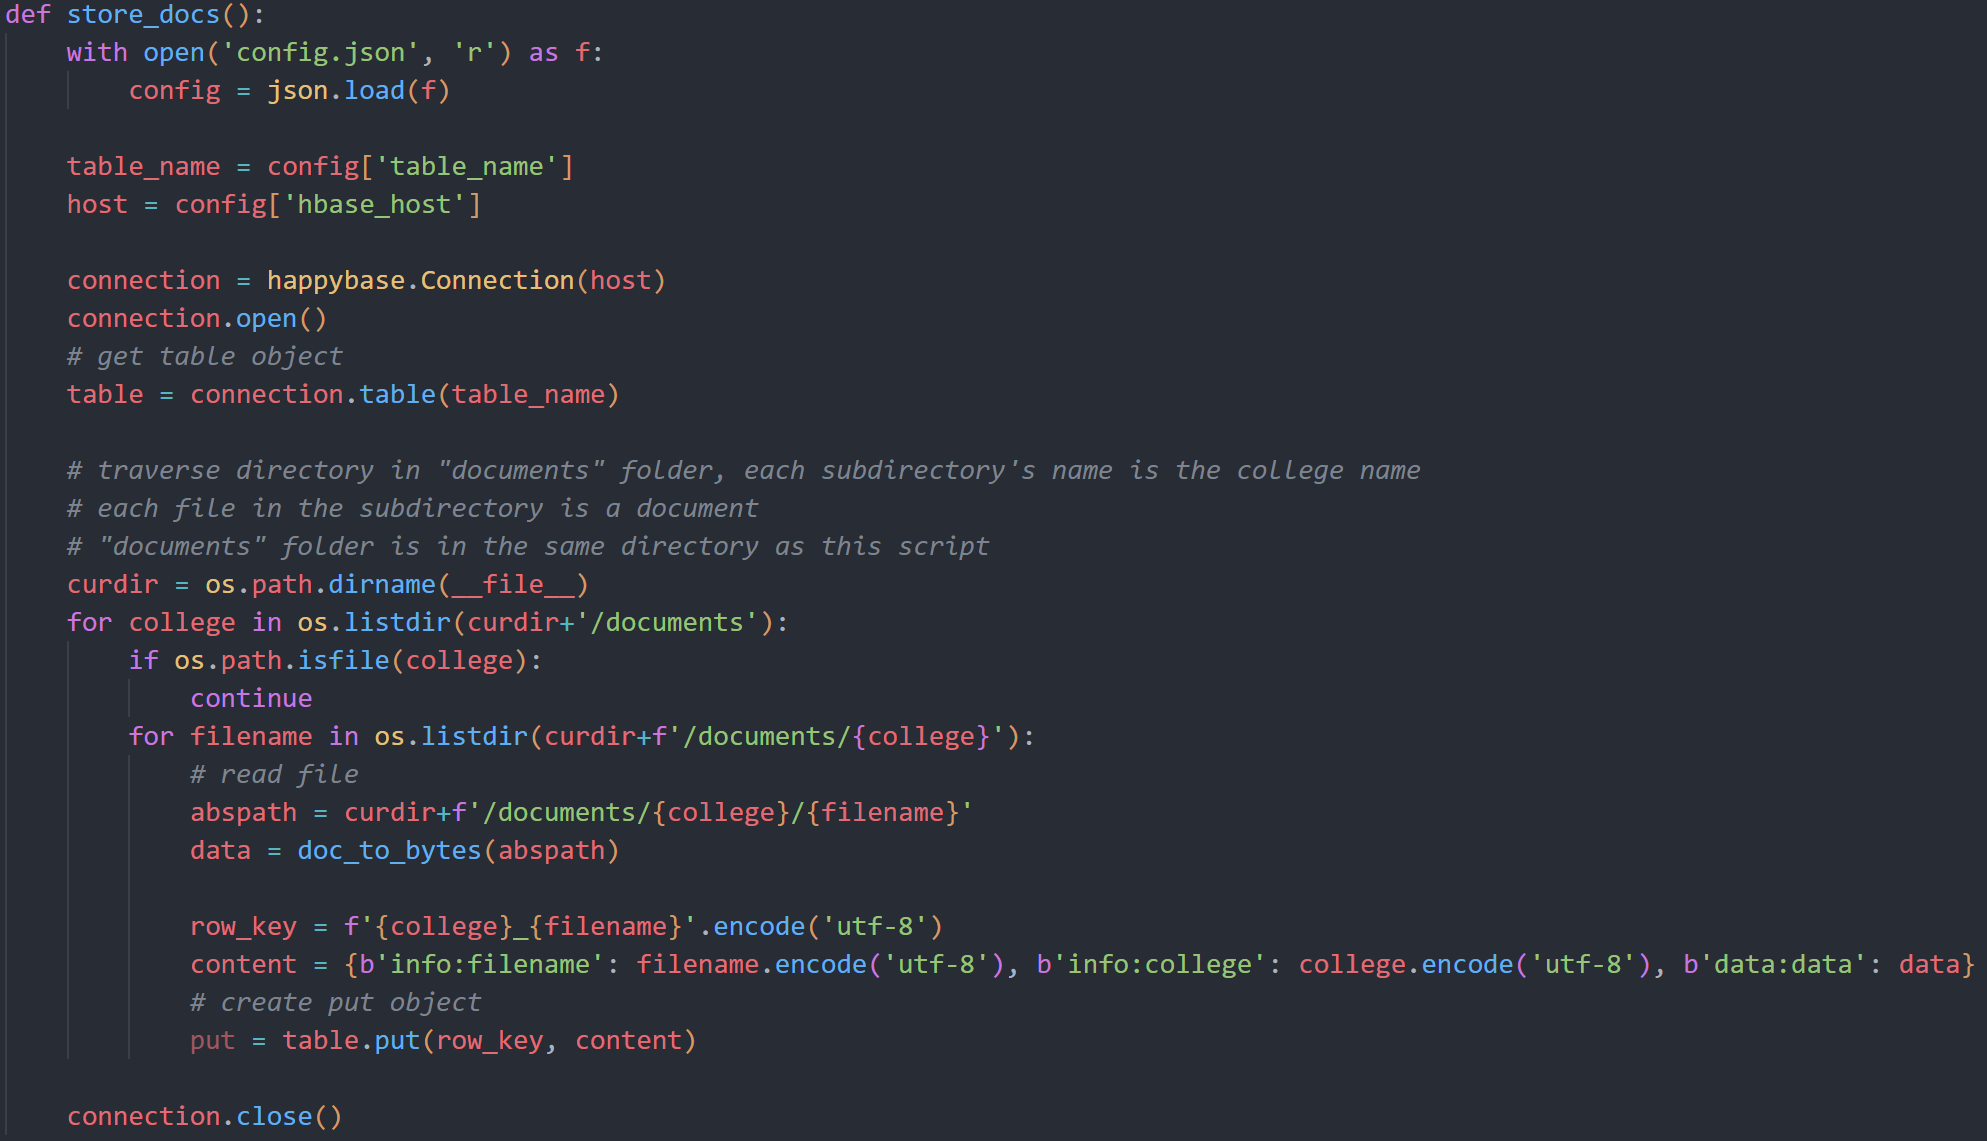
\includegraphics[width=0.6\linewidth]{store}
		\caption{存储文件}
		\label{fig:store}
	\end{figure}
	\subsection{排序}
	考虑到需要按照相似性进行排序,因此选择TfidfVectorizer进行文本特征提取以计算余弦相似度。主要使用habbybase的scan函数遍历表选择符合条件的文件,随后通过tfidf值计算余弦相似度来的到相似性排序。在这个过程中,主要耗时在于遍历和计算tfidf值。后续优化的思路,一是在遍历时使用多线程,二则是选择更高效的文本特征提取方法。
	\begin{figure}[h]
		\centering
		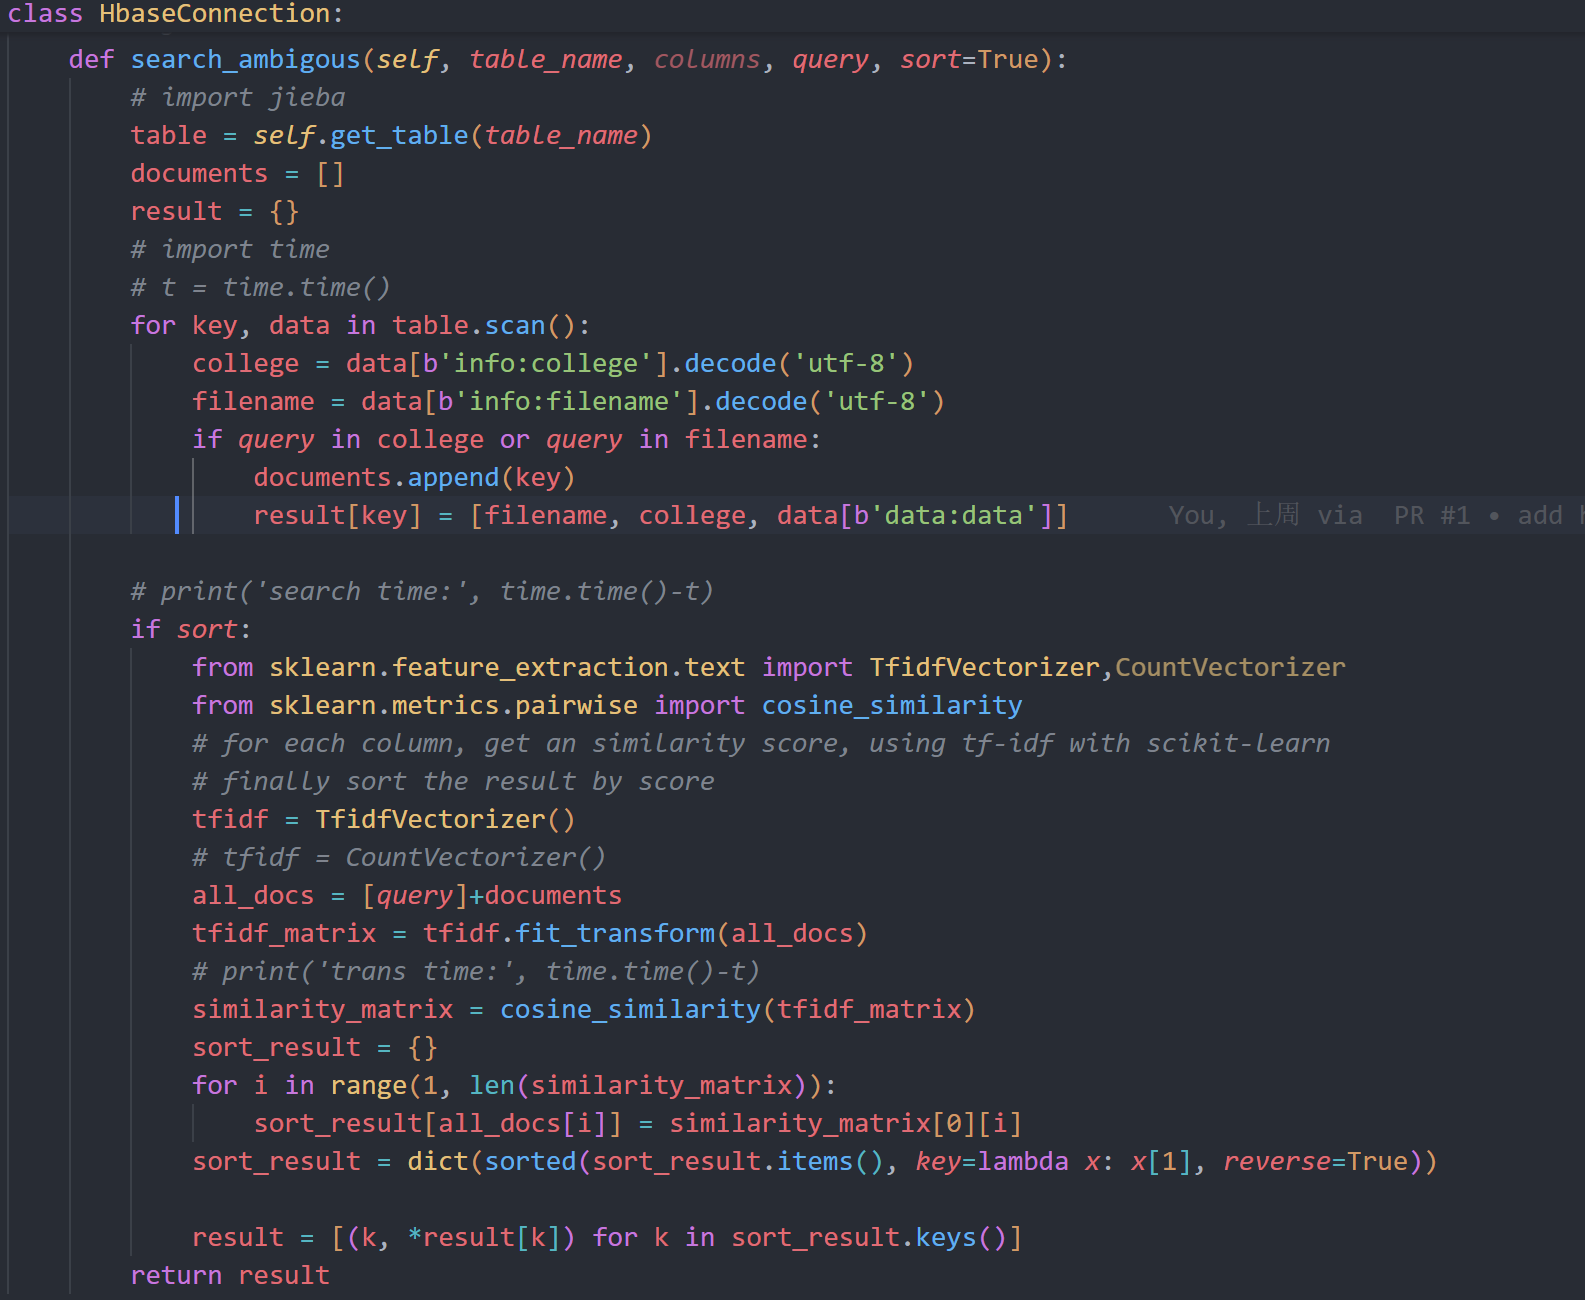
\includegraphics[width=0.6\linewidth]{sort}
		\caption{搜索}
		\label{fig:sort}
	\end{figure}
	
	\section{使用说明}
	\subsection{依赖}
	项目开发环境为Python 3.9,需要安装happybase、PyQt5等第三方库。
	此外若需要使用检索结果相关性排序功能,需要安装scikit-learn等库。
	
	\subsection{文件}
	本部分介绍如何存储爬取的文件,以及从数据库下载到本地的文件,请参照附录\ref{附录}中的文件结构。
		\begin{enumerate}
			\item
			爬取的文件需要按照学院分类存储,每个学院的文件存储在一个以学院名命名的文件夹中。
			然后分别将这些文件夹存储在\texttt{initialization/documents}目录下。
			\item
			系统运行时检索并下载到本地的文件会存储在\texttt{document\_output}目录下。
			用户可以自行决定是否保留这些文件。
		\end{enumerate}
	
	\subsection{方法}
	完成环境安装后,先运行start\_hbase.py以启动软件,在将导入文件按要求放置完毕后允许initialize.py文件完成建表和数据导入,最后运行main.py文件,在显示的搜索界面进行搜索。使用完毕后,运行stop\_hbase.py文件以终止运行。
	
	
	\section{效果展示}
	\begin{figure}[h]
		\centering
		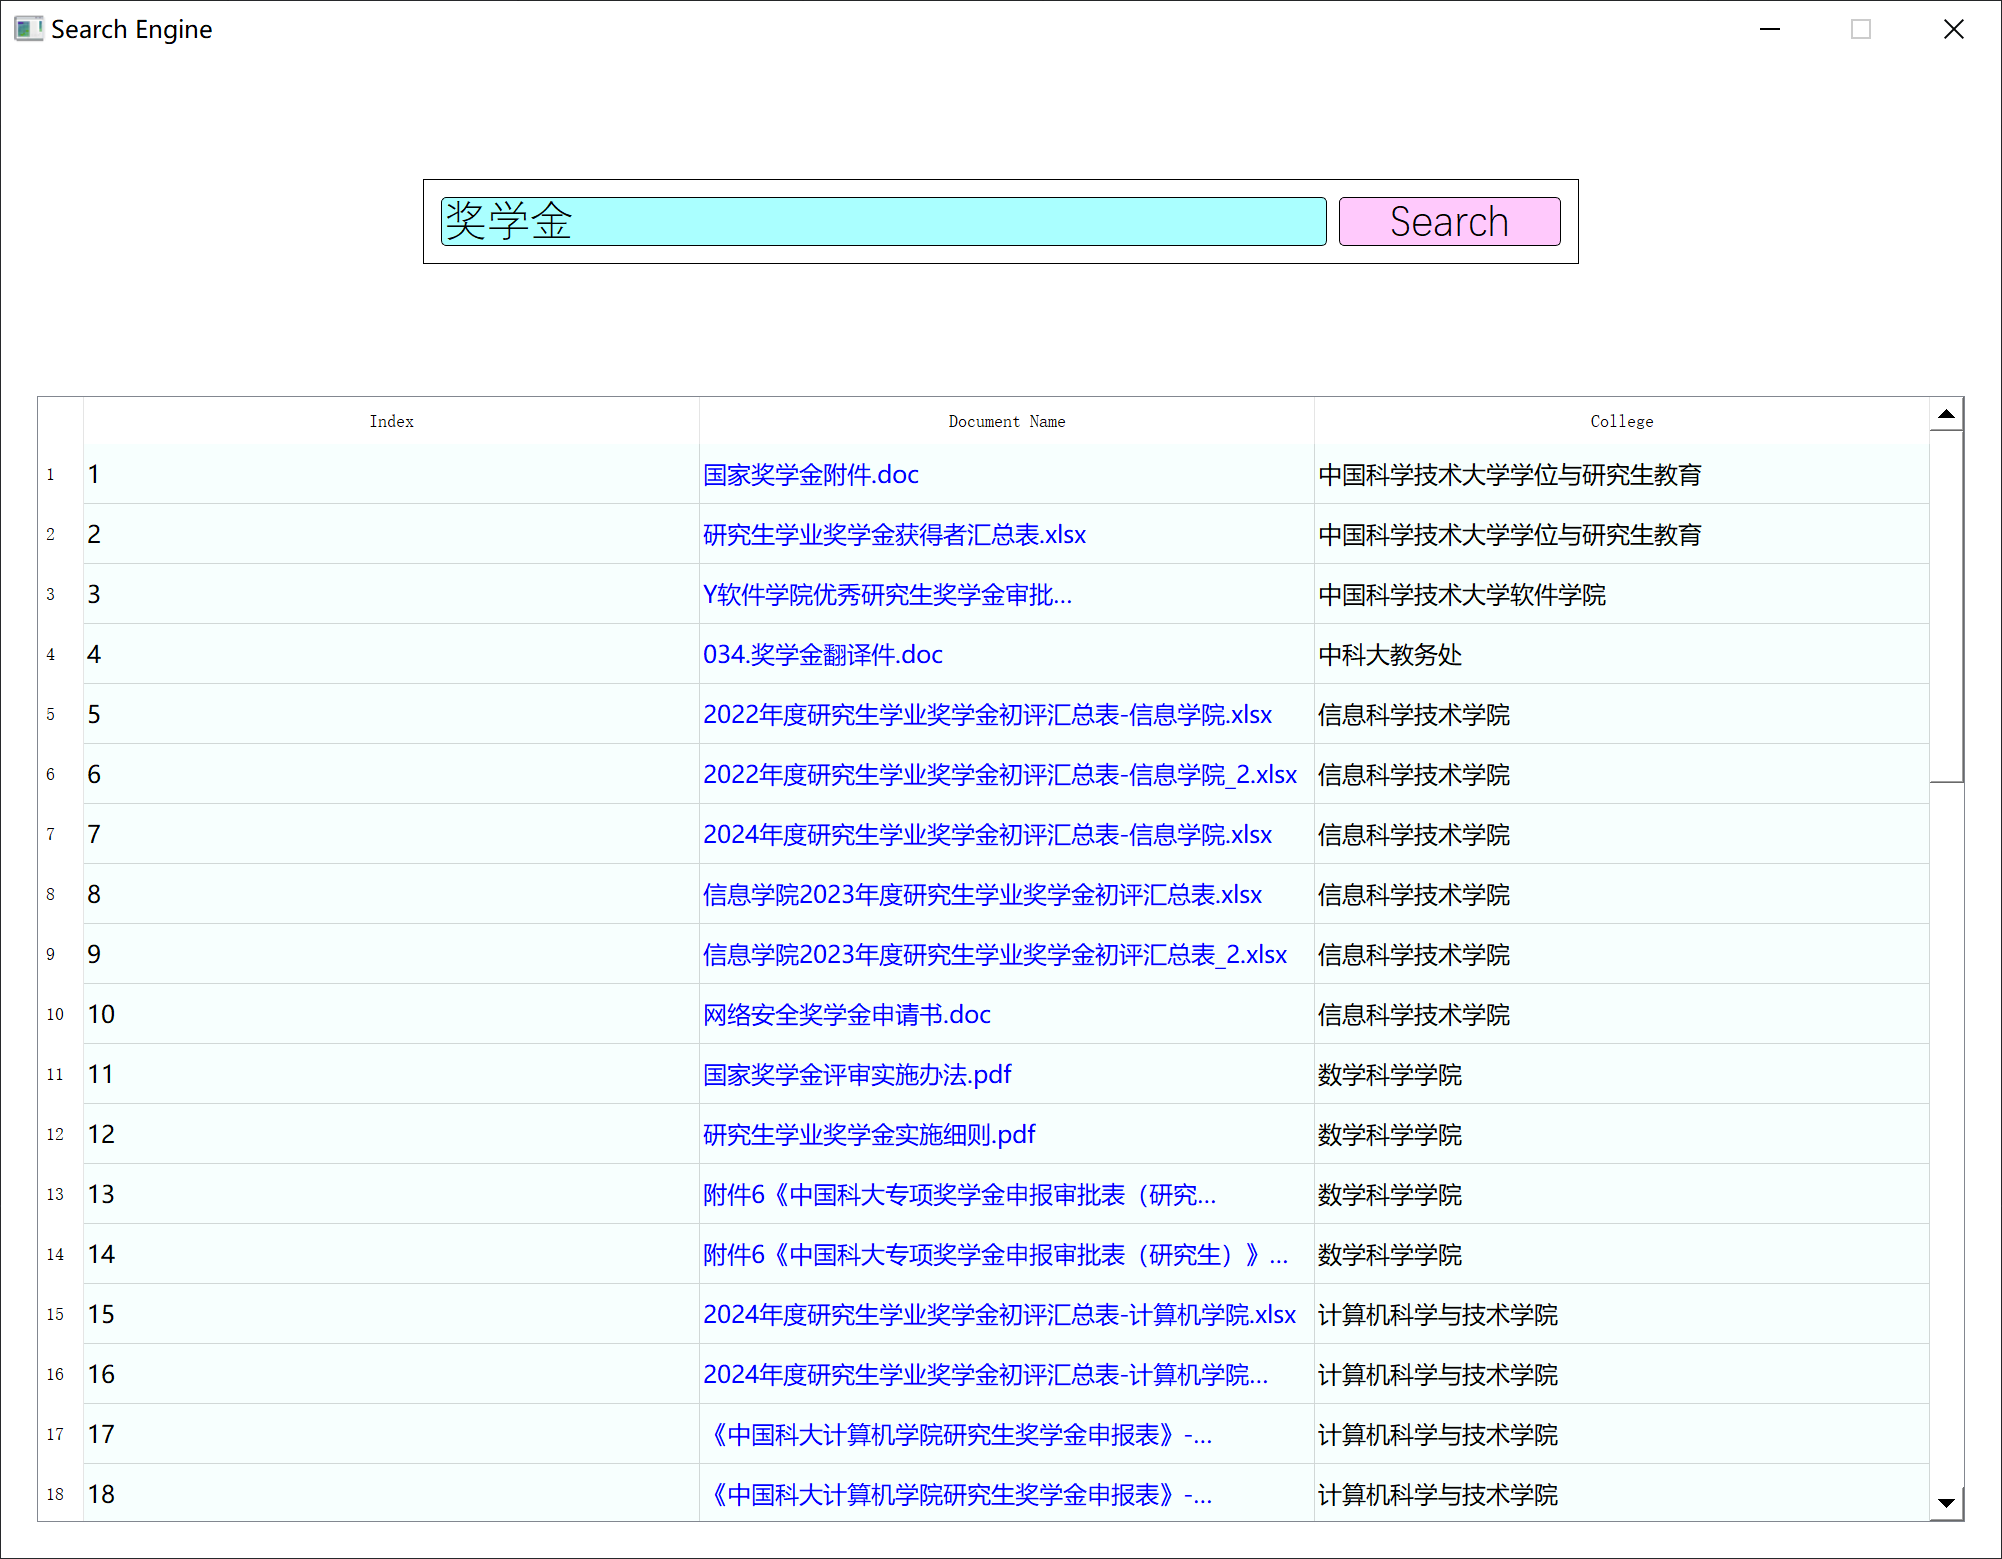
\includegraphics[width=0.4\linewidth]{screenshot001}
		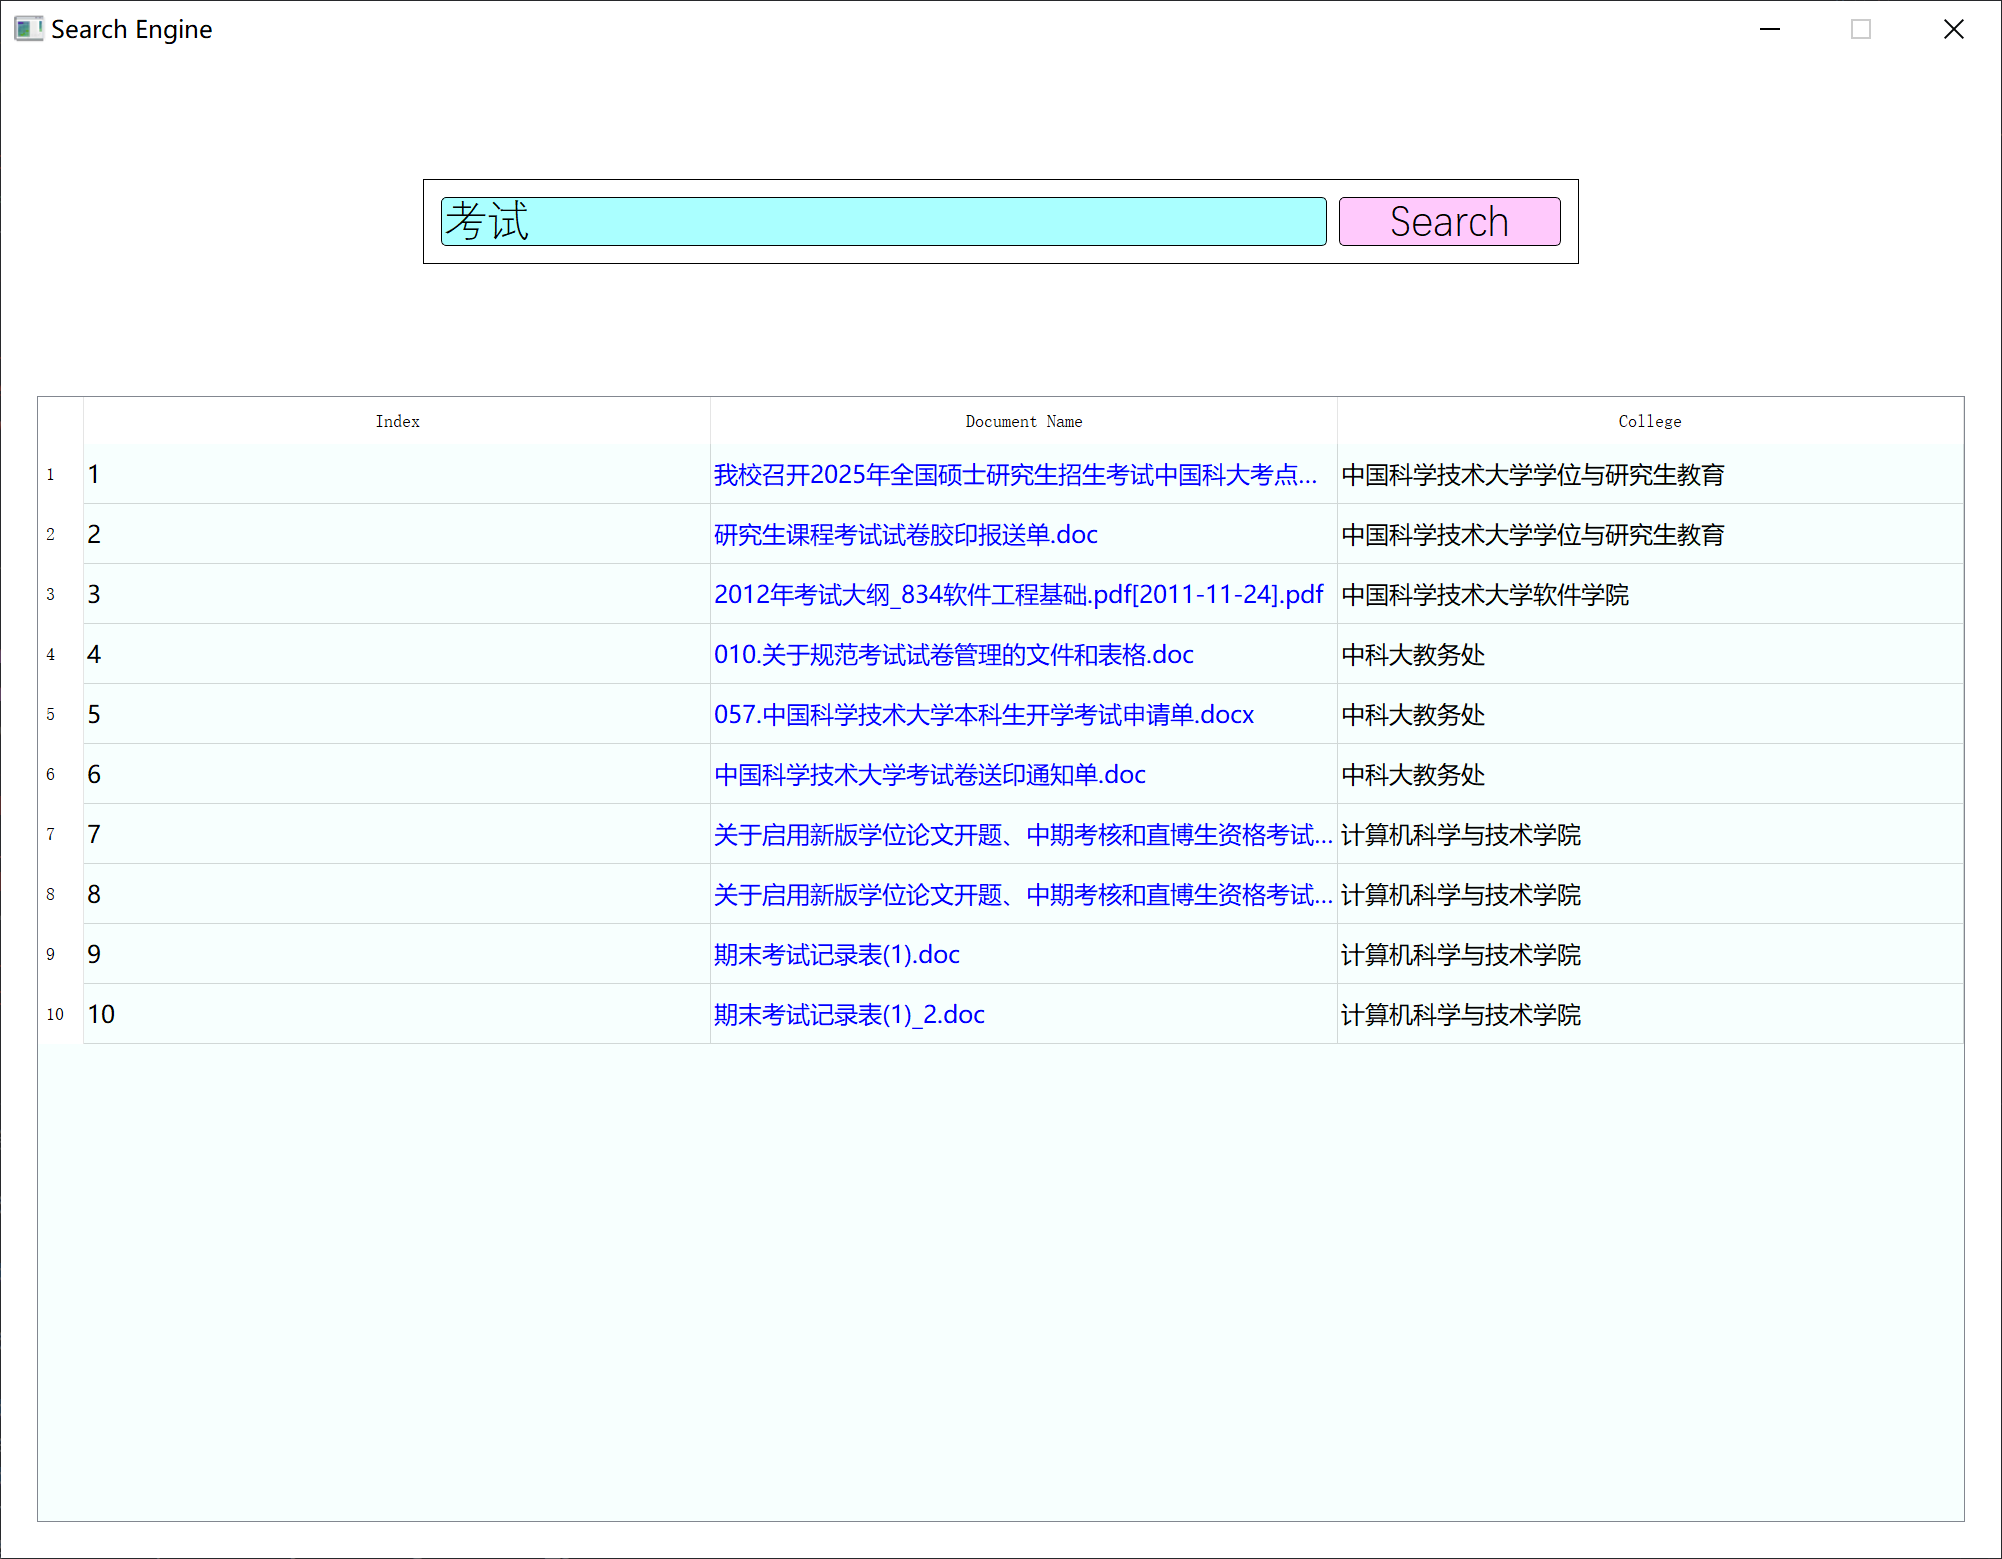
\includegraphics[width=0.4\linewidth]{screenshot002}
		\caption{搜索效果演示}
		\label{fig:screenshot001}
	\end{figure}
	
	\section{成员分工}
	\begin{itemize}
		\item 殷腾PB20030785:项目整体框架搭建,前端图形化界面设计。
		\item 李新涛PB21151754:文件爬取与环境准备、数据库表设计及排序搜索。
	\end{itemize}
	

	\section*{附录}\addcontentsline{toc}{section}{附录}
	\begin{center}
		\begin{minipage}{0.5\textwidth}
			\dirtree{%
				.1 /.
					.2 crawl.
						.3 \_\_init\_\_.
						.3 crawler.py.
						.3 grad.py.
						.3 mathematics.py.
						.3 press.py.
						.3 scs.py.
						.3 sist.py.
						.3 sse.py.
						.3 teach.py.
					.2 document\_output.
					.2 initialization.
						.3 documents.
						.3 create\_table.py.
						.3 store\_docs.py.
						.3 initializa.py.
					.2 report.
						.3 report.pdf.
						.3 report.tex.
					.2 scripts\_hbase.
						.3 config\_hbase.json.
						.3 start\_hbase.py.
						.3 stop\_hbase.py.
					.2 uis.
						.3 \_\_init\_\_.py.
						.3 mainwindow.py.
						.3 ui\_mainwindow.py.
						.3 ui\_warningwindow.py.
						.3 warningwindow.py.
					.2 utils.
						.3 \_\_init\_\_.py.
						.3 docs.py.
						.3 hbase.py.
					.2 config.json.
					.2 crawl\_data.
					.2 main.py.
					.2 README.md.
			}
		\captionof{table}{项目文件结构}
		\label{附录}
		\end{minipage}
	\end{center}
	
\end{document}